\section{Fundamentação Teórica}

\subsection{Codificação de Cores}
\begin{frame}
    \begin{columns}
        \begin{column}{0.5\textwidth}
            \begin{figure}
                \centering
                \caption*{RGB}
                \begin{tikzpicture}[radius=1.5cm]

    \coordinate (O) at (0,0);
    
    % \draw [help lines, dashed] (-3,-3) grid (3,3); % desenha grid
    % \draw [red] (O) node[draw,cross out] {}; % marca pont(0,0) 
    
    % \path[fill=Black] (-2.5,-2.5) rectangle (2.5,2.5);
    \path[draw=rgb_K, fill=rgb_K] circle[radius=3cm];
    % \clip (-6.8,-4) rectangle (6.8,4);

  % \draw (0,0)  arc[start angle=180, end angle=90]
  %     (2,.5) arc[start angle=90,  delta angle=-90];
  % \draw (4,0) -- +(30:1cm)
  %             arc [start angle=30,  delta angle=30] -- cycle;
  % \draw (8,0) arc [start angle=0,   end angle=270,
  %                  x radius=1cm, y radius=5mm] -- cycle;

    % \path[draw, fill=green] (150:1) arc[start angle=180, end angle=90];
    
    \coordinate (cG) at (90 :0.866);
    \coordinate (cR) at (210:0.866);
    \coordinate (cB) at (330:0.866);

    % \path[draw=green, thick] (cG) circle;
    % \path[draw=red,   thick] (cR) circle;
    % \path[draw=blue,  thick] (cB) circle;

    \path[draw=rgb_R, fill=rgb_R]
        (cR) arc (240:180:1.5)
        arc (120:300:1.5)
        arc (240:180:1.5)
    ;

    \path[draw=rgb_G, fill=rgb_G]
        (cG) arc (120:60:1.5)
        arc (0:180:1.5)
        arc (120:60:1.5)
    ;

    \path[draw=rgb_B, fill=rgb_B]
        (cB) arc (0:-60:1.5)
        arc (-120:60:1.5)
        arc (0:-60:1.5)
    ;

    \path[draw=rgb_C, fill=rgb_C]
        (cG) arc (120:60:1.5)
        arc (0:-60:1.5)
        arc (0:60:1.5)
    ;
    
    \path[draw=rgb_M, fill=rgb_M]
        (cB) arc (0:-60:1.5)
        arc (240:180:1.5)
        arc (240:300:1.5)
    ;
    
    \path[draw=rgb_Y, fill=rgb_Y]
        (cR) arc (240:180:1.5)
        arc (120:60:1.5)
        arc (120:180:1.5)
    ;

    \path[draw=rgb_W, fill=rgb_W]
        (cB) arc (0:60:1.5)
        arc (120:180:1.5)
        arc (240:300:1.5)
    ;
    

    
\end{tikzpicture}
                \caption*{Fonte: Autor.}
            \end{figure}
        \end{column}
        \begin{column}{0.5\textwidth}
            \begin{figure}
                \centering
                \caption*{CMYK}
                \begin{tikzpicture}[radius=1.5cm]

    \coordinate (O) at (0,0);
    
    % \draw [help lines, dashed] (-3,-3) grid (3,3); % desenha grid
    % \draw [red] (O) node[draw,cross out] {}; % marca pont(0,0) 
    
    % \path[fill=Black] (-2.5,-2.5) rectangle (2.5,2.5);
    \path[draw=cmyk_K, dashed, fill=cmyk_W] circle[radius=3cm];
    % \clip (-6.8,-4) rectangle (6.8,4);

  % \draw (0,0)  arc[start angle=180, end angle=90]
  %     (2,.5) arc[start angle=90,  delta angle=-90];
  % \draw (4,0) -- +(30:1cm)
  %             arc [start angle=30,  delta angle=30] -- cycle;
  % \draw (8,0) arc [start angle=0,   end angle=270,
  %                  x radius=1cm, y radius=5mm] -- cycle;

    % \path[draw, fill=green] (150:1) arc[start angle=180, end angle=90];
    
    \coordinate (cG) at (90 :0.866);
    \coordinate (cR) at (210:0.866);
    \coordinate (cB) at (330:0.866);

    % \path[draw=green, thick] (cG) circle;
    % \path[draw=red,   thick] (cR) circle;
    % \path[draw=blue,  thick] (cB) circle;

    \path[draw=cmyk_C, fill=cmyk_C]
        (cR) arc (240:180:1.5)
        arc (120:300:1.5)
        arc (240:180:1.5)
    ;

    \path[draw=cmyk_Y, fill=cmyk_Y]
        (cB) arc (0:-60:1.5)
        arc (-120:60:1.5)
        arc (0:-60:1.5)
    ;

    \path[draw=cmyk_M, fill=cmyk_M]
        (cG) arc (120:60:1.5)
        arc (0:180:1.5)
        arc (120:60:1.5)
    ;

    \path[draw=cmyk_R, fill=cmyk_R]
        (cG) arc (120:60:1.5)
        arc (0:-60:1.5)
        arc (0:60:1.5)
    ;
    
    \path[draw=cmyk_G, fill=cmyk_G]
        (cB) arc (0:-60:1.5)
        arc (240:180:1.5)
        arc (240:300:1.5)
    ;
    
    \path[draw=cmyk_B, fill=cmyk_B]
        (cR) arc (240:180:1.5)
        arc (120:60:1.5)
        arc (120:180:1.5)
    ;

    \path[draw=cmyk_K, fill=cmyk_K]
        (cB) arc (0:60:1.5)
        arc (120:180:1.5)
        arc (240:300:1.5)
    ;
    

    
\end{tikzpicture}
                \caption*{Fonte: Autor.}
            \end{figure}
        \end{column}
    \end{columns}
\end{frame}

\subsection{Visão Computacional}
\begin{frame}
    \begin{columns}
        \begin{column}{0.5\textwidth}
            \begin{figure}
                \centering
                
\includegraphics[width=0.9\textwidth]{../pictures/OpenCV_Logo_with_text.png}
                \caption*{Fonte: \href{https://commons.wikimedia.org/wiki/File:OpenCV_Logo_with_text.png}{Adi Shavit, Public domain, via Wikimedia Commons}}
            \end{figure}
        \end{column}
        \begin{column}{0.5\textwidth}
            \begin{figure}
                \centering
                
\includegraphics[width=1\textwidth]{../pictures/Tesseract_OCR_logo_(Google).png}
                \caption*{Fonte: \href{https://commons.wikimedia.org/wiki/File:Tesseract_OCR_logo_(Google).png}{Google, Inc., Public domain, via Wikimedia Commons}}
            \end{figure}
        \end{column}
    \end{columns}
\end{frame}

\subsection{Banco de Dados sobre Medicamentos}
\begin{frame}
    \begin{figure}
        \centering
        \caption*{Página de campos de consulta ao Bulário Eletrônico da Anvisa.}
        \label{fig:bulario_pagina}
        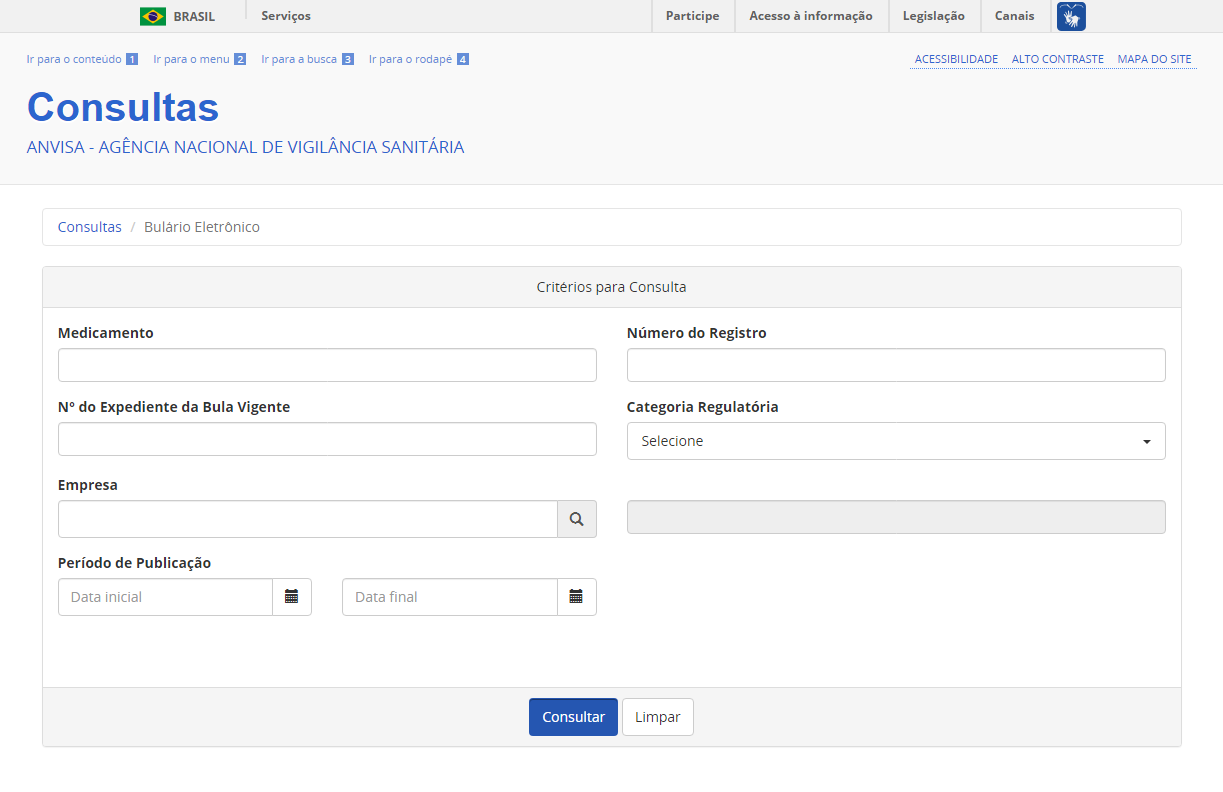
\includegraphics[width=0.85\textwidth]{../pictures/bulario_pagina.png}
        \caption*{Fonte: \href{https://consultas.Anvisa.gov.br/\#/bulario/}{Portal da Anvisa}, acesso em 2023-09-06.}
    \end{figure}
\end{frame}
